\begin{auf}
    647
\end{auf}
Eine rechteckige Leiterschleife (Länge $l=8cm$, Breite $b=5cm$) befindet sich in einem homogenen Magnetfeld mit der Flussdichte $B=0.12T$.
\begin{enumerate}
    \item[a] Wie groß ist der magnetische Fluss $\Phi$ durch die Schleife, wenn \textbf{B} und die Flächennormale \textbf{A} einen Winkel von $30^\circ$ einschließen?
    \item[b] Wie groß ist die maximale induzierte Spannung, wenn die Schleife im Magnetfeld mit einer Winkelgeschwindigkeit von $\omega=100s^{-1}$ rotiert?
    \item[c] Welche Spannung wird induziert, wenn die Schleife so durch das Feld
    bewegt wird, dass \textbf{B} parallel zu \textbf{A} ist?
\end{enumerate}
\begin{figure}[h]
    \centering
    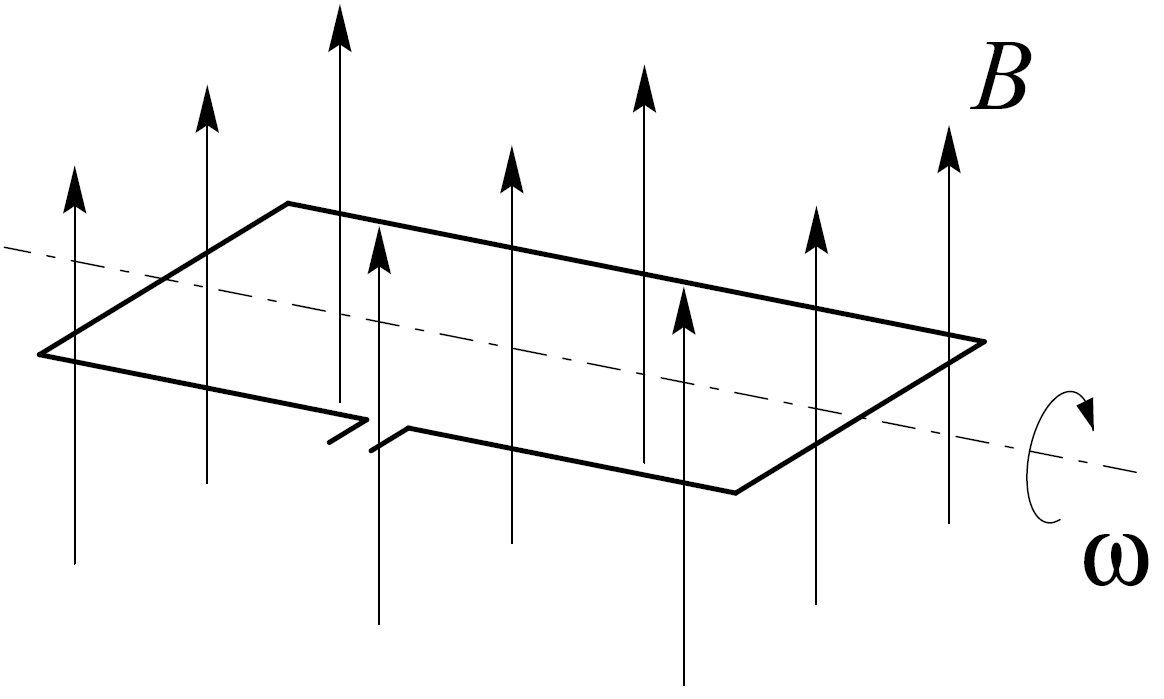
\includegraphics[width=0.7\linewidth]{images/647_0.png}
    \caption{Versuchsaufbau Aufgabe 647}
\end{figure}